\documentclass[11pt,a4paper]{article}




\usepackage{amsmath, bm, fancyhdr, graphicx, environ, chemformula, tabu, multirow, booktabs, pgfplots, blindtext, xcolor, indentfirst, lastpage, pgfplotstable, datatool, float, setspace, textgreek, makecell, newfloat, tabu, csquotes, subcaption, threeparttable}

\usepackage{tabularx}
\newcolumntype{Y}{>{\centering\arraybackslash}X}
\newcolumntype{Z}{>{\raggedright\arraybackslash}X}
\newcolumntype{P}[1]{>{\centering\arraybackslash}p{#1}}

\usepackage[image={scale=0.75}]{chemschemex}

\usepackage{siunitx}
\sisetup{detect-all, round-pad = false, round-mode=places, round-precision=4}
\DeclareSIUnit[quantity-product = {}]\calorie{cal}
\usetikzlibrary{shapes.geometric, arrows, calc}
\pgfplotsset{compat=1.18}


\newcommand{\SIvar}[3][]{%
\DTLgetvalueforkey{\sitemp}{thevalue}{python_variables}{thekey}{#2}%
\SI[#1]{\sitemp}{#3}}

\newcommand{\NumVar}[1]{%
\DTLgetvalueforkey{\sitemp}{thevalue}{python_variables}{thekey}{#1}%
\num{\sitemp}}

\newcommand{\Var}[1]{%
\DTLgetvalueforkey{\sitemp}{thevalue}{python_variables}{thekey}{#1}%
\sitemp}

\usepackage[hidelinks]{hyperref}
\usepackage[english]{babel}
\usepackage[super]{nth}
\usepackage[backend=biber, style=chem-angew, articletitle=true]{biblatex}
\renewbibmacro*{date}{\printtext[parens]{\printtext[date]{\printdate}}}
\DeclareFieldFormat[article]{title}{#1}
\DeclareFieldFormat[article]{volume}{#1}
\AtEveryBibitem{%
  \clearfield{note}%
}

\usepackage[labelfont=bf]{caption}
\captionsetup{labelsep=period, font={stretch=1.5, footnotesize}, justification=justified, singlelinecheck=false} 

\textwidth 16cm
\textheight 24cm
\topmargin -2.7cm
\oddsidemargin 0.25cm
\parindent 0pt

\newcommand{\mean}[1]{\langle #1 \rangle}

\newcommand{\tabitem}{~~\llap{\textbullet}~~}

\DeclareFloatingEnvironment[
  fileext = los ,
  listname = {List of Schemes} ,
  name = Scheme
]{scheme}

\setcellgapes{2.5pt}

\widowpenalty10000
\clubpenalty10000
\newcommand{\pKa}{\mathrm{pK}_a}
\addbibresource{References/references.bib}
\begin{document}

% -------- only change entries beginning here ----------------------------
%
% choose language of coverpage: german or english
\newif\ifeng
\engtrue
%\engfalse

% If you want colored links, hyperref must be changed in the preamble
% If the names for the following entries are too long, break them into several
% lines using \\
%
% enter the title 
\def\title{VL - Advanced Organic Technology I}
%
% enter studentid
\def\id{11802845 \\ 11816060}
% enter your mail
\def\mail{k11802845@students.jku.at \\ k11816060@students.jku.at}
%
\def\study{Script}
%\def\study{Electrochemistry Laboratory}
%
% enter your name
\def\name{Diana Drachsler}
%
% for the german version you also have to enter the sex (male or female)
\newif\ifsupvismale
\supvismaletrue
%\supvismalefalse
%
% enter course name
\def\course{317.014}
%
% enter month year or \today for the today's date
\def\date{\today}

\def\protocoldate{\today}

\def\students{Fabian Hofmann}
\graphicspath{{Figures/}}



% do not change anything below this line
% -------------------------------------------------------------------------------
%
\pagestyle{empty}

\makeatletter
\def\Huge{\@setfontsize\Huge{25pt}{30}}
\makeatother
%
\unitlength 1cm
%\sffamily
\begin{picture}(16.7,0)
\ifeng
 \put(11.5,-2.5){
\includegraphics[width=5.2cm]{jku_en}}
\else
 \put(11.5,-2.5){
\includegraphics[width=5.2cm]{jku_de}}
\fi
\put(11.9,-4.2){\begin{minipage}[t]{3.9cm}\footnotesize%
\ifeng
 Written by\\
\else
 Verfasst von\\
\fi
{\bfseries\name}%
 \vskip 4mm%
 \ifeng
  Course\\
 \else
  Kurs\\
 \fi
 {\raggedright\bfseries\course}%
\vskip 4mm
 Date\\
{\bfseries\date}

\end{minipage}}
\put(12.9,-25){\begin{minipage}[t]{3.9cm}\footnotesize%
{\bfseries JOHANNES KEPLER\\
\ifeng
 UNIVERSITY
\else
 UNIVERSIT\"AT
\fi
LINZ}\\
Altenbergerstra{\ss}e 69\\
4040 Linz, \"Osterreich\\
www.jku.at\\
DVR 0093696
\end{minipage}}
\put(0,-12.2){\begin{minipage}[b]{11cm}\raggedright\Huge\bfseries\title\end{minipage}}
\put(0,-17.2){
\includegraphics[width=4.4cm]{arr}}
\put(0,-18.3){\begin{minipage}[t]{12cm}%
{\Large\study}
\vskip 4mm
Editor: {\students}
\end{minipage}}
\end{picture}

\setstretch{1.5}

\newpage

%%%%%%%%%%%%%%%%%%%%% Header Config %%%%%%%%%%%%%%%%%%%%%

\pagestyle{fancy}
\setlength\headheight{2.4cm}
\lhead{}
\rhead{
\includegraphics[scale=0.15]{jku_en.pdf}}
\lfoot{\today}
\cfoot{Advanced Organic Technology I}
\rfoot{\thepage /\pageref*{LastPage}}

%%%%%%%%%%%%%%%%%%%%% Introduction %%%%%%%%%%%%%%%%%%%%%

%\tableofcontents
%\listoffigures
%\listoftables
%%%
%\section*{List of Symbols}
%%
%\begin{tabularx}{\linewidth}{XXX}
%      $S_{ymbol}$ & unit & description\\
%    \end{tabularx}
%\newpage

\section*{Preface}
I would like to thank Dominik Böhm for the very detailed summary of the lecture material including the incorporation of the additional information from the lecture.
I have made it my task to digitise the 101 pages of the handwritten summary including all illustrations.
This will make it easier for students in future years to incorporate changes in the lecture content.
The \LaTeX~script can be downloaded from my GitHub page.
I wish everyone good luck with the IMHTA exam.

\vspace{0.5cm}

Fabian Hofmann

\newpage

\tableofcontents

\newpage
%---------------------------------------------------------------%
\part{Refinery and Fuels}
Crude oil (\SI{33.6}{\percent}), coke (\SI{27.2}{\percent}) and gas (\SI{23.9}{\percent}) are still the 3 main energy sources, followed by hydropower (\SI{6.8}{\percent}), nuclear power (\SI{4.4}{\percent}) and renewable energy sources (\SI{4}{\percent}).

Crude oil is the most important energy source due to its ease of extraction, wide range of applications and cheap transport.

\subsection{Kerogen}
Kerogen is an organic waxy material found in sedimentary rocks and formed from bacteria, decayed algae and wood.
It is the most common form of organic carbon in the earth.
Kerogen can be converted into synthetic oil at temperatures above \SI{500}{\celsius} or by hydration.
Canada (Athabasca Oil Sands) has the world's largest deposit of kerogen.
This deposit is close to the surface, making surface mining the primary method of extraction.
In this region mining of the oil sands dates back to 1967.
The worlds top reserve holders are China, United States, Argentina, Mexico, South Africa, Australia and Canada.

\subsubsection{Types of kerogen}
Kerogen can be divided into four different types.

\paragraph{Typ I (Sapropelic)}
Sapropelic kerogen contains the highest amount of oil and is therefore the most promising source.
It is derived form algea and its proteins and lipids.
It contains only few cyclic or aromatic structures.
Type I kerogen has high initial hydrogen-to-carbon ratios (H/C > 1.25) and low initial oxygen-to-carbon ratios (O/C < 0.15).

\paragraph{Type II (Planktonic)}
Planktonic kerogen is mostly based on marine organic materials.
It has a hydrogen-to-carbon ratio H/C smaller than 1.25 and initial oxygen-to-carbon ratio O/C of 0.03 to 0.18.

\paragraph{Typ III (Humic)}
Type III kerogens are characterized by low initial H/C ratios and high initial O/C ratios.
Type III kerogens are derived from terrestrial plant matter, specifically from precursor compounds including cellulose, lignin, terpenes and phenols.
Coal is an organic-rich sedimentary rock that is composed predominantly of this kerogen type.
On a mass basis, type III kerogens generate the lowest oil yield of principal kerogen types.
It has a hydrogen-to-carbon ratio H/C smaller than 1 and initial oxygen-to-carbon ratio O/C of 0.03 to 0.3.

\paragraph{Type IV (Residue)}
Type IV kerogen comprises mostly inert organic matter in the form of polycyclic aromatic hydrocarbons.
They have no potential to produce hydrocarbons
It has a hydrogen-to-carbon ratio H/C smaller than 0.5.

\subsection{Fracking}
Fracking is a method of creating, widening and stabilising cracks in the rock of a reservoir deep underground with the aim of increasing the permeability of the reservoir rocks.
This allows gases or liquids in them to flow more easily and steadily to the wellbore and be extracted.

In fracking, the fracking fluid is injected through a well under high pressure, typically several hundred bar, into the geological horizon from which it is to be extracted.
The fracking fluid is water, which is usually mixed with proppants, such as silica sand, thickeners and further additives.
Usually, several deviated wells (lateral wells) are first drilled into the reservoir by means of directional drilling, whereby the drill bit is guided parallel to the layers.
This means that the available borehole length in the reservoir is much greater, which generally increases the production yield.
Further additives are:

\begin{itemize}
    \item Gels (e.g. guar) to increase the viscosity of the fluid for better sand transport
    \item Foams (\ch{CO2} or \ch{N2}) for better transport and deposition on the proppant
    \item Acids (HCl, \ch{CH3COOH}, HCOOH, \ch{H3BO3}) for the dissolution of minerals
    \item Furthermore: Corrosion inhibitors, viscosity adjusters, biocides, fluid loss additives (preventing loss of fluid into neighboring rocks), friction minimizers
\end{itemize}

\subsection{Oil drilling}
Traditional methods of oil extraction have been the primary and secondary methods, which only exhaust between a quarter and half of a well’s oil reserves.
Such profligacy has been addressed by the development of a tertiary technique, more commonly known as enhanced oil recovery (EOR).

\subsubsection{Primary methods}
Primary oil recovery refers to the process of extracting oil either via the natural rise of hydrocarbons to the surface of the earth or via pump jacks and other artificial lift devices.
Since this technique only targets the oil, which is either susceptible to its release or accessible to the pump jack, this is very limited in its extraction potential.
Only around \SIrange{10}{20}{\percent} the well’s potential are recovered from the primary method.

\subsubsection{Secondary methods}
This method involves the injection of gas or water, which will displace the oil, force it to move from its resting place and bring it to the surface.
This is typically successful in targeting an additional \SI{30}{\percent} of the oil’s reserves.

\subsubsection{Tertiary methods (Enhanced Oil Recovery)}
Rather than simply trying to force the oil out of the ground, as did the previous two methods, enhanced oil recovery seeks to alter its properties to make it more conducive to extraction.
Tertiary methods target more than \SI{50}{\percent} of the oil’s reserves.
There are three main types of enhanced oil recovery

\paragraph{Thermal recovery}
This is the most prevalent type of EOR and works by heating the oil to reduce its viscosity and allowing easier flow to the surface.
This is most commonly achieved by introducing steam into the reservoir, which will work to heat the oil.

\paragraph{Gas injection} 
Either natural gas, nitrogen or carbon dioxide (increasingly the most popular option) are injected into the reservoir to mix with the oil, making it more viscous, whilst simultaneously pushing the oil to the surface (similar to secondary oil recovery).

\paragraph{Chemical injection}  
Polymers or surfactans are used to free trapped oil in the well.
This is done by lowering surface tension and increasing the efficiency of water-flooding.

\subsection{Crude Oils and Products}
\label{subsec:crude_oils_and_products}
Crude oil contains great variety of hydrocarbons (HCs).
There are three types of molecular structures are possible straight-chain, branched-chain and ring structures (Fig.~\ref{fig:hc_structs}).

\begin{figure}[H]
    \centering
    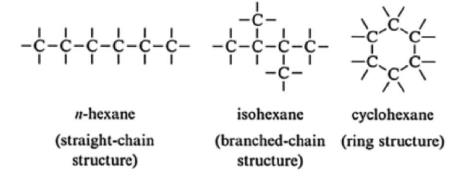
\includegraphics{Figures/HC_structures}
    \caption{Different possible hydrocarbon structures}
    \label{fig:hc_structs}
\end{figure}

\subsubsection{Categorization of Crude Oil}

\paragraph{Based on structure} Crude oils are complex mixtures primarily composed of hydrocarbons (HCs).
These hydrocarbons can be categorized into several groups, including saturated hydrocarbons, unsaturated hydrocarbons, aromatics, and heteroorganic compounds.

\subparagraph{Saturated hydrocarbons} They are also known as paraffins or alkanes, make up a significant portion of crude oils.
They can be further classified into normal, iso-, and cycloalkanes.
Cycloalkanes, often referred to as naphthenes, are a subgroup of saturated hydrocarbons characterized by their ring-shaped structure.

\subparagraph{Unsaturated hydrocarbons} These are in the form of olefins or alkenes.
They are not typically present in significant quantities in crude oils.
However, they can be formed during various refining processes, such as cracking and dehydrogenation.

\subparagraph{Aromatic hydrocarbons} Crude oils also contain varying amounts of aromatic hydrocarbons, including benzene, condensed polynuclear aromatics, and aromatic ring systems with various paraffinic or olefinic side chains.
Aromatics are not only naturally occurring but can also be formed in different conversion processes within the oil industry.

In addition to hydrocarbons, crude oils may contain heteroorganic compounds, albeit in relatively small concentrations.
These compounds include organic molecules containing sulfur (S), nitrogen (N), and oxygen (O), as well as trace quantities of metal compounds like vanadium (V), iron (Fe), and nickel (Ni).

Crude oils can be categorized based on the types of hydrocarbons they contain, leading to three primary classifications: paraffin-based, naphthene-based, and mixed-based crude oils.

\subsubsection{Paraffin-Based Crude Oils}
These crude oils are characterized by a predominant presence of paraffinic hydrocarbons.
Within this category, the lower and medium molecular weight paraffins are particularly valuable.
They are well-suited for a wide range of catalytic conversion processes, resulting in the production of gasolines, middle distillates, and serving as essential chemical feedstocks.
On the other hand, the higher molecular weight paraffins are typically utilized as raw materials for the manufacture of lubricating oils and paraffin waxes.

\subsubsection{Naphthene-Based Crude Oils}
Naphthene-based crude oils primarily consist of naphthenic, aromatic, and asphaltic hydrocarbons.
The lower and medium molecular weight components present in these crude oils are instrumental in producing high-quality gasoline components, solvents, and act as key feedstocks for the production of aromatic compounds.
In contrast, the higher molecular weight components in naphthene-based crude oils find application in the manufacturing of specialized lubricants and in the production of bitumen.

\subsubsection{Mixed-Based Crude Oils}
Mixed-based crude oils represent a diverse group with an even distribution of paraffinic and naphthenic/aromatic hydrocarbons across all molecular weight ranges.
They constitute the largest class of crude oils.

Crude oils can also be classified according to the product fractions they yield.
This classification distinguishes between light, medium, and heavy crudes, and it is primarily based on the proportions of distillates and residues within the crude oil.
In essence, the more atmospheric residues a crude oil contains, the heavier it is considered in this categorization.

Light crude oils are characterized by a higher proportion of distillates, making them relatively easier to refine and yielding a larger quantity of valuable, lighter products such as gasoline and diesel fuel.
They are often preferred for their economic and operational advantages in the refining process.

Medium crude oils strike a balance between distillates and residues.
They contain a moderate amount of atmospheric residues and distillates.
This category can provide a diverse range of refined products, including not only gasoline and diesel but also heavier products like kerosene and lubricating oils.

Heavy crude oils, on the other hand, have a higher proportion of atmospheric residues, making them more challenging to refine.
They typically yield a significant amount of heavier products, including bitumen and heavy fuel oils.
These crudes are often characterized by their high viscosity and density, requiring more complex and energy-intensive refining processes.
%---------------------------------------------------------------%

\printbibliography

%\setcounter{section}{0}
\renewcommand\thesection{\Alph{section}}
\section{Appendix}\label{appendix}



\end{document}
